\documentclass[12pt]{article}

\usepackage{graphicx}
\usepackage{subcaption}

\begin{document}
\title{\textbf{Eye of Mordor} \\Sparktech}
\maketitle

\section{Team members}
\begin{itemize}
\item Miguel Rodriguez
\item Shao-Wen Chang
\item Asadujaman Nur
\item Vincent Obigwe
\end{itemize}

\section{Introduction}

The population of human civilization is increasing rapidly. With this growing population, we need many lands for farming, resident and industrial purposes. Thus, we have been chopping down the forests to support this huge demand for the lands. Although it is solving many problems for us, it is creating many issues by endangering the animal life and forcing them to relocate their natural habitats, which leads them to move closer and closer to people and our habitat. Which causes unexpected fatal accidents.

The problem we are facing is, due to lack of their natural habitats, they, for example deer, are living near firms and woods. In addition, sometime they like to hide or take shelter from people if they get scared or are if they are injured. Sometime they sleep and rest inside those lands.  Which can be a huge problem. Since they are deep inside the firming lands, the firmer and the animal rescuers do not know their stances; therefore they cannot provide support or perform rescue operation in case they are in need of support. Even worst, during the harvesting season, if they are injured(Animals) and decides to have shelter inside the fields such as corn ones and cannot move due to their injuries or too weak, and farmers starts to harvest the corps, sometimes they just run over their tractor on the poor animals without knowing their presence and killing them as a result. This can be avoid by the help of technology. 

To solve this issue and save the wildlife, we are going to develop a system, which will detect the animals hiding inside the fields and transmit the data to a receiver to either the farmer or the animal rescuer. So that they can take necessary action to save their life. Here in this project we are going to develop a prototype model using sensors and micro controllers to approach this problem. We will discuss more about the components we will use, methods and implementation in details below.


\section{Concept Description}

\begin{figure}[!h]
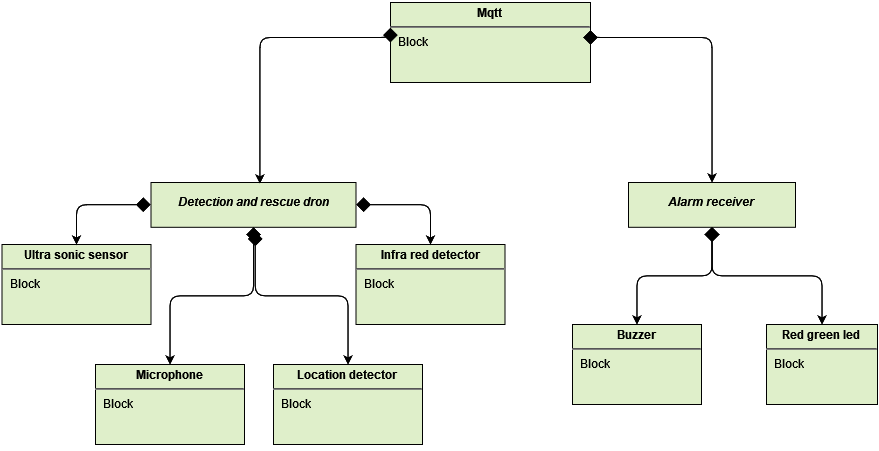
\includegraphics[scale=0.6]{img/block_diagram.png}
\caption{Block Diagram}
\label{fig::bd}
\end{figure}

The project has three main components, a Raspberry pi 3B that works as the broker, an Arduino Uno Wifi Rev 2, that acts as the transmitter and the receiver, and a mobile phone that is able to receive the data produced by the broker, and also return an acknowledgement command. Figure \ref{fig::bd}. 

The the devices, the Raspberry pi, the Arduino Uno and the mobile are connected to the same LAN network, in some cases we can also use the mobile phone as a hotspot to interconnect the other two devices. Fig \ref{fig::broker}.

\begin{figure}[!h]
\centering{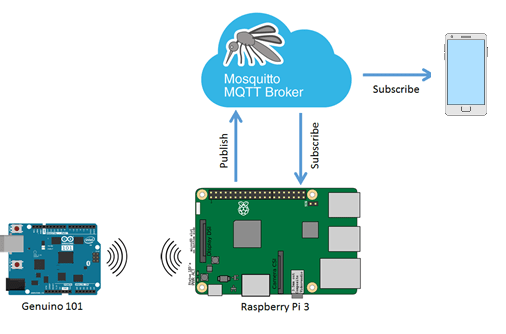
\includegraphics[scale=1]{img/mosquitto1.png}}
\caption{Broker connection through LAN}
\label{fig::broker}
\end{figure}

On the Raspberry Pi 3 we installed Mosquitto, the broker that will receive the information proceeding from the sensors, analyse this data and return the calculated results to both the mobile phone and the Arduino Uno, that depending on the received data will behave in different ways that will be deeply explained in section \ref{sec:implementation}.

The Arduino Uno is equipped with an ultrasonic sensor, that will act as the detector for animals. For the purposes of the simulation was not possible to use all the desired sensor. The Arduino is also connected with five leds: while to let us visualize the Wifi connection, the white led will be static on when the Wifi connection is not working and it will blink when the connection is established. The blue led will keep on when the broker is disconnected, and it will turn of when the broker is connected. The green led is on when the detections are far from the sensor or there is not a detection, in the case of our simulation more than 12 cm, the yellow led will turn on when the detection is between 6 and 12 cm, and when the detection is smaller than 6 cm both the red led and a buzzer to simulate an alarm system. The alarm then can be silenced with the acknowledge button on the mobile app. The schematics of the connection Arduino can be seen on Figure \ref{fig::ard}

\begin{figure}[!h]
\centering{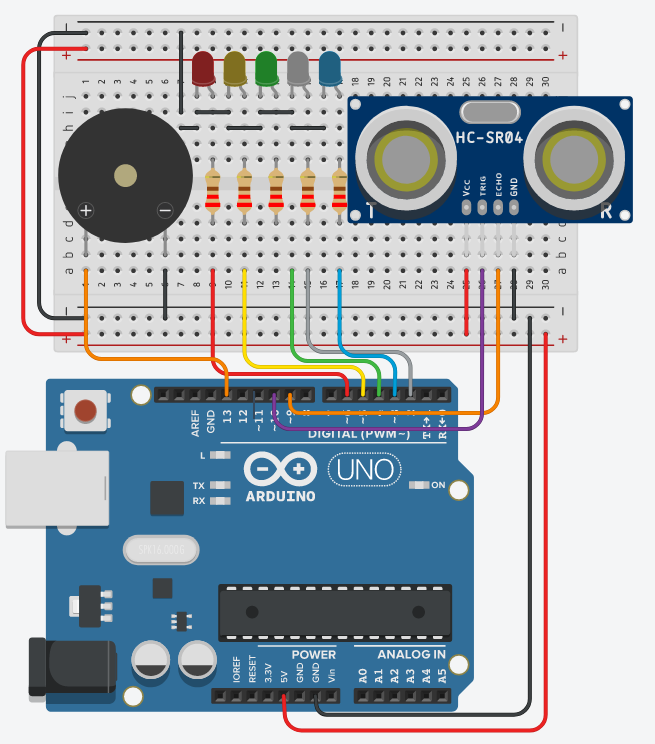
\includegraphics[scale=0.6]{img/tinker1.png}}
\caption{Schematics of Arduino connections}
\label{fig::ard}
\end{figure}

\section{Project / Team management}

In carrying out our project, we consider project management as an important aspect that helps us in realizing the goal and objective faster. Project management benign the application of various methods, skill knowledge and experience to achieve a detailed object that has already been set and marked as the project acceptance benchmark. It is also very important that time and budget are considered. As students we embarked on this project with the focus on managing time and delivering the best result given the limited amount of time that and the no budget we deal with.  Having this in mind, we decided to approach the whole project using the agile project management. 

Agile project management is known as an iterative means of delivering a project throughout a given life cycle. There life cycle are made up of several iterations that are all geared towards the completion of the project. This leads to us having weekly meetings to analyze tasks and evaluate progress. With Agile project management, continuous improvement and development is the goal, to enable the project to get better on further iterations. While using Agile project management, we made use of Kanban framework to be able to achieve our project. 

Kanban is a framework on agile project management that is deals with growth changes and the need for continuous process improvement. The core practices involved in using Kanban are: 

1.	Visualization of tasks in a board like manner with tools such as excel. 

2.	Reduction of work in project by introducing changes incrementally.

3.	Management of the flow of to-dos.

4.	Defining processes and tasks clearly.

5.	Enhancing the process of feedback to enable improvement of the system.

6.	Improving work flow all together. 

To be able to properly visualize our tasks and clearly see what each member of the group has to do, we made use of GitHub projects. GitHub projects can be seen as a customizable spreadsheet that helps us integrate tasks with GitHub in our repository. It empowers more customization by enabling filtering; sorting, grouping and working with GitHUb pull requests. It further looks static with the addition of colors to determine the various stage each task is. 


\section{Technologies}

In this section, we explained the technologies used in our project. We split the technology into two namely hardware and software. The reason for the split is due to the fact that our project contains both software and hardware components that are linked to work together. Fig \ref{fig::architecture} 

\begin{figure}[!h]
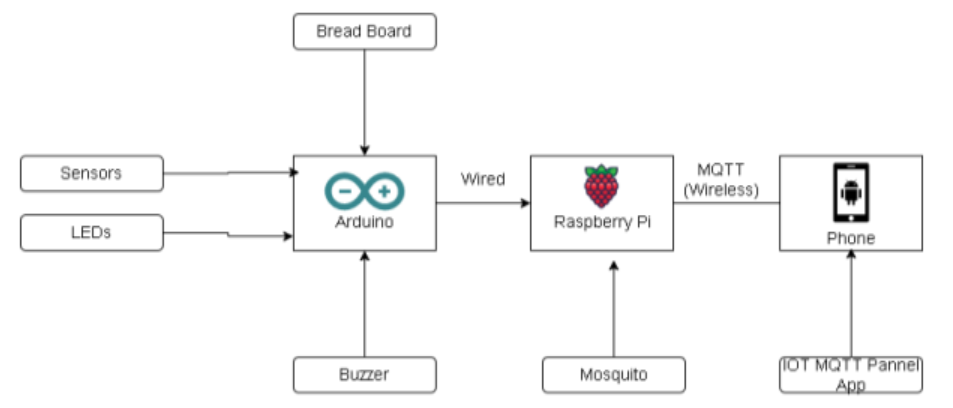
\includegraphics[scale=0.55]{img/architecture.png}
\caption{System Architecture}
\label{fig::architecture}
\end{figure}

As can be seen by the diagram above which explains the basic connection between the sensors, led, Arduino raspberry pi, phones, etc. This will further be explained in the forthcoming subsections. 

\subsection{Hardware} 

In carrying out our project, a wide range of hardware was used in accomplishing the task. The hardware components used include but are not limited to:

\subsubsection{Sensors}

We made use of a wide range of sensors such as ultrasonic sensors that enables us to detect when a farm instrument is approaching the animal.

\subsubsection{Buzzer}

The buzzer acts as an actuator that informs the farmer of an animal's presence. The buzzer produces a sound that acts as a signal.

\subsubsection{Breadboard}

A breadboard is a tool/device that is used to seamlessly connect wires and other supporting electronic components while prototyping \cite{tech1}. Since the Eye of Mandor is a prototype, made use of breadboard to connect the sensors, resistors, etc with the Arduino.

\subsubsection{Led}

In our project, LED is used to signify the position of the tractor or farming device to an animal or obstruction. The light turns GREEN when there is no obstruction or the tractor is nowhere close. YELLOW when there is a construction, but the farming instrument is still in far proximity to the animal. The light turns RED when it is now in close proximity to the animal.

The LED serves as an additional precaution with the buzzer to offer multiple layers of protection for the animal.

\subsubsection{Arduino}

Arduino is an open-source platform that is commonly used in the process of building and programming electronics. It has the capability of sending and receiving information from devices \cite{tech2}.

In our project, Arduino was used to connecting all the sensors, buzzers,s and the rest of the electric component. It transmits the data to the Raspberry Pi through a wired connection.

\subsubsection{Raspberry Pi} 

Raspberry Pi is a low-cost mini-computer that was developed by the Raspberry Pi Foundation UK. It can serve as a computer CPU and perform various computer functions \cite{tech3}. In our project, Raspberry Pi was used for a wide range of tasks which includes installing a mosquito for a connection with the mobile phone through MQTT and getting data from the Arduino.

\subsubsection{Phone}

The mobile phone was used to establish a connection with the Rasberry Pi wirelessly using MQTT. This is done through software.

\subsection{Software} 

There are also software components of our application. The software includes but is not limited to:

\subsubsection{Mosquitto} 

Mosquitto is a popular opensource MQTT broker that permits the process of connecting to sensors, devices, and apps in publish and subscribe architectures \cite{tech4}. In our project, a mosquito was used as the MQTT broker. It was installed on the raspberry pi.

\subsubsection{MQTT Protocol}


Message Queuing Telemetry Transport (MQTT) is an open publish and subscribe protocol that is designed for constrained devices and is used for telemetry purposes [5]. In our project, MQTT was used with the help of mosquitoes to connect to the mobile app in a subscribe and publish manner.

\subsubsection{IoT MQTT Panel App}


This is an android application that enables us to subscribe to and publish topics through the MQTT protocol. This app communicated with the Rasberry pi with the help of mosquito which is installed in the raspberry pi. 

\section{Implementation} \label{sec:implementation}

There were three main components to implement Eye of Mordor, the Arduino, the Raspberry Pi and the MQTT mobile app.

\subsection{Raspberry Pi}

To realize the connection between client and server, the first step was to install Mosquitto broker in the Raspberry Pi. By default. A broker program written in C++ runs on the Raspberry pi to decode information under the MQTT protocol. The c broker on the Raspberry Pi has two functions \textit{on\_connect} and \textit{on\_message}. The \textit{on\_message} function handles all the incoming messages from the Arduino, it makes the computation and then return the value of the LED which has to be turned on or off as well when the buzzer buzzes. Figure \ref{fig::broker}

\begin{figure}[!h]
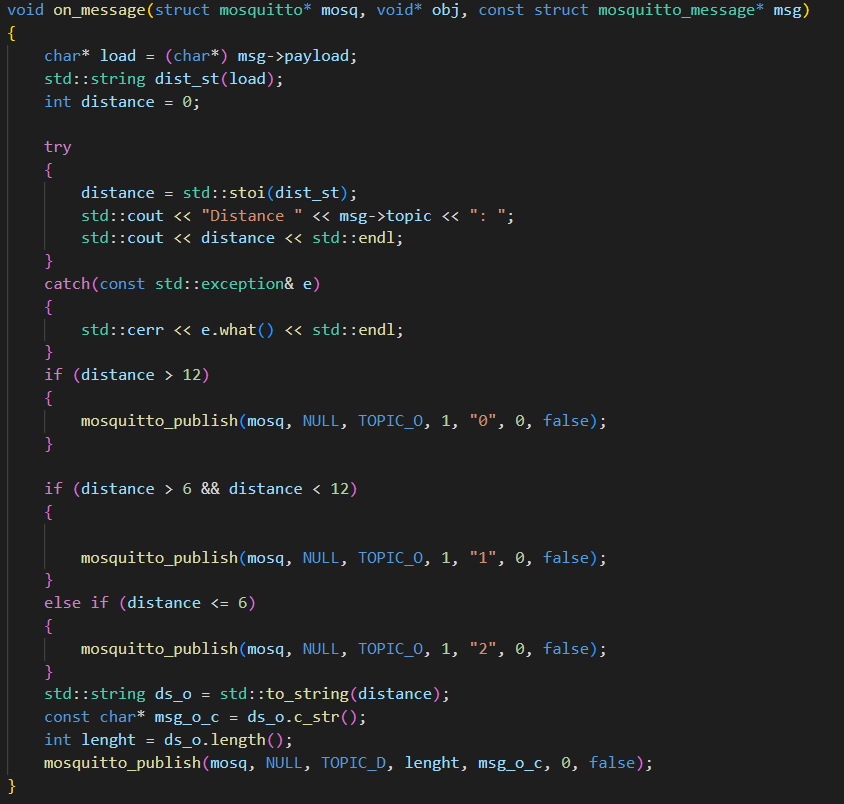
\includegraphics[scale=0.665]{img/broker.png}
\caption{C++ broker}
\label{fig:broker}
\end{figure}

\subsection{Arduino} \label{sec:arduino}

The implementation in the Arduino starts with the connection to the the Internet, this connection was done with the use of the WiFiNINA library, we declare the IP address of the broker and the port that we will use. The IP address can be taken from the command line on the Raspberry Pi with the command \textit{hostname -I}, and the port is defined as \textit{1883} that is the port defined by the Mosquitto broker. We also define the names of the topics that are used in the implementation: \textit{uss, led} and \textit{stop}. The \textit{uss} topic will send the information of the ultra sonic sensor, the \textit{led} topic will receive the information of which led has to be on and the \textit{stop} topic is used to stop the buzzer using the mobile phone. Moreover, the ports of the Arduino are setted as shown in Figure \ref{fig:arduino1}.

\begin{figure}[h]
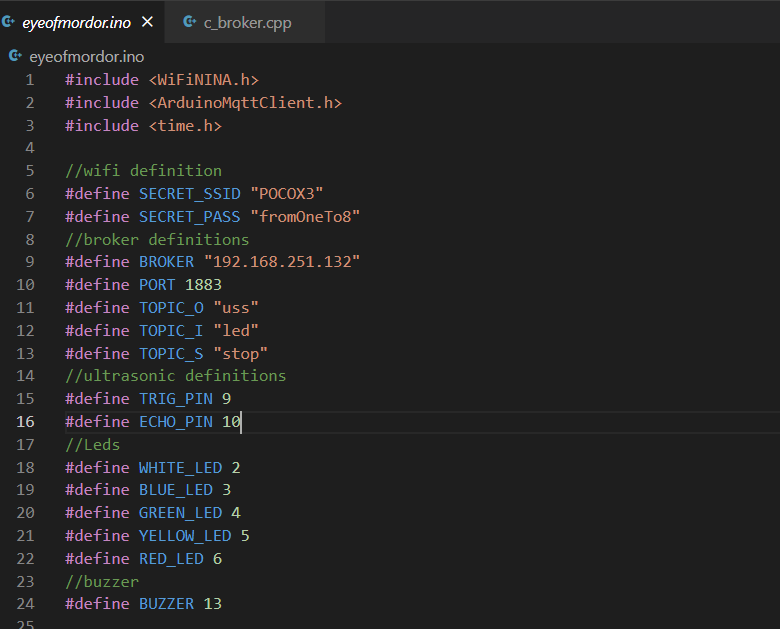
\includegraphics[scale=0.665]{img/ard1.png}
\caption{Arduino configuration}
\label{fig:arduino1}
\end{figure}

We define three states that will represent the distance of the detection, the first state for detections farther than 12 cm, the second for detections between 6 and 12 cm and the third one for detections closer than 6 cm. The initial state is state 1 as we supposed that at the first moment there will not near detection Fig \ref{fig:arduino2}.

\begin{figure}[h]
\centering{ 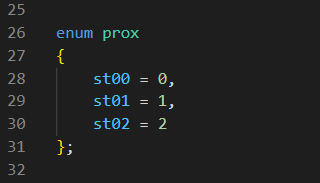
\includegraphics[scale=0.7]{img/ard2.png}}
\caption{Arduino states}
\label{fig:arduino2}
\end{figure}

The Arduino code is based in six functions \textit{wifisetup(), onMqttMessage(int messageSize), ultrasonic\_pub(), reconect(), setup()} and \textit{loop()}. The \textit{wifiesetup} function is in charge to connect with the wifi connection as well to connect with the broker and to subscribe to the different topics, the \textit{ultrasonic\_pub}  function is in charge of publish the information of the ultra sonic sensor through the \textit{uss} topic. The \textit{reconnect} function will be called in case that the broker or the wifi connection fail and will reconnect the system. the \textit{onMqttMessage(int messageSize)} function get the information coming from the different topics and process it, this function, depending on the received message will change the status of the system, turn on or turn of the different leds and turn on or turn off the buzzer depending on the communication with the Raspberry pi and the mobile app. The \textit{setup} function is a basic Arduino function where we set up our board ant the \textit{loop} function is also a basic Arduino function where we run an infinite loop, this function will call in an infinite loop the publisher and the subscriber. It also checks if the connection is still active, in case is not active will call the \textit{reconnect} function.

\subsection{MQTT Mobile app}

The MQTT mobile app is configured with the IP address, and the port with the same data used in the Arduino (Section \ref{sec:arduino}). The mobile app subscribes only to the topic \textit{distance} to get the distance of the detections, and publishes in the topic \textit{stop} to stop the buzzer when beeping when the detection is still close to the sensor.

\begin{figure}[h]
\centering{ 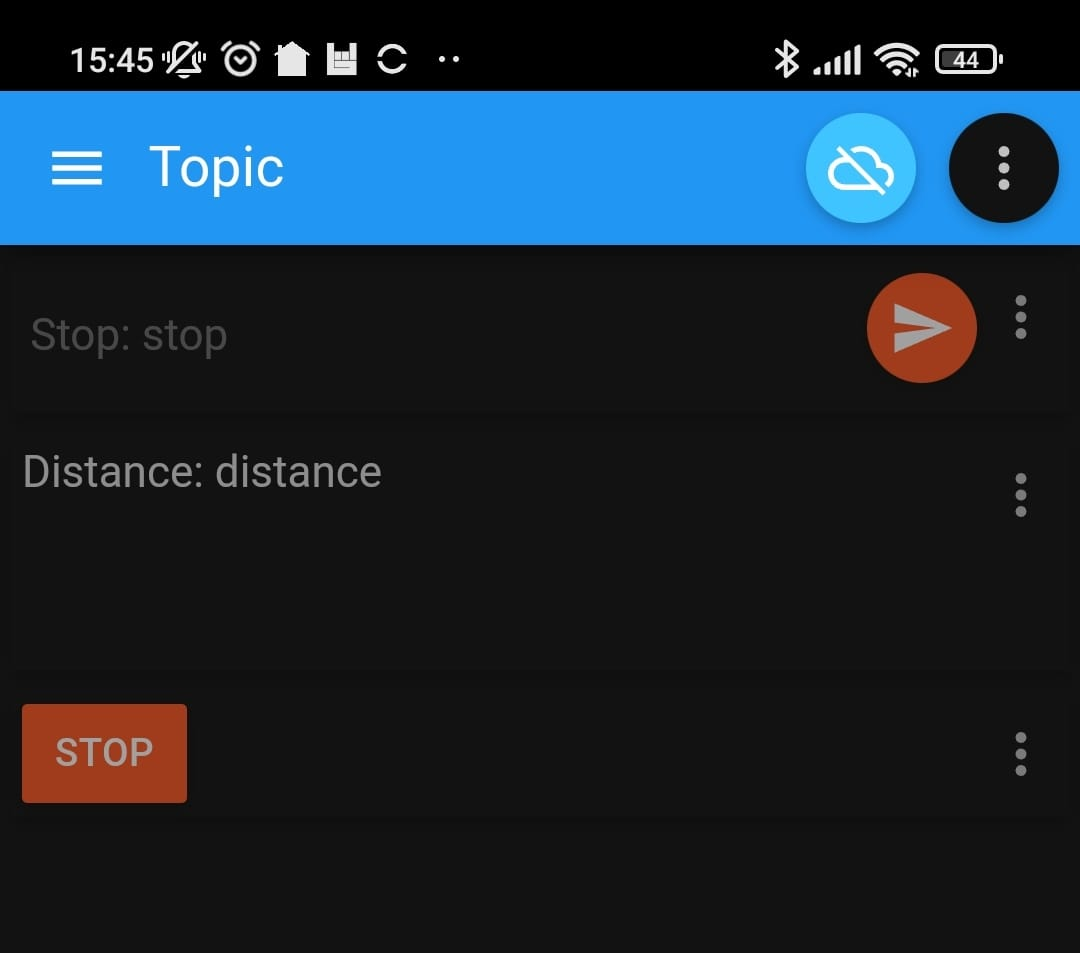
\includegraphics[scale=0.25]{img/phone1.jpeg}}
\caption{Mobile app}
\label{fig:phone1}
\end{figure}


\section{Use Cases}

From the previous sections, we got to learn all the technical method and the technologies that being used to realize the project. Here in this section we will talk more about how the project can be realize in real life scenarios.

As discussed in “Introduction and Concept” Sections, We are trying to Develop a system that can be used to save and rescue animal life hiding inside field from unwanted accident primarily. Which can

be extended later on to help and assist in resque operation in search of lost human and animal in the wilderness aswell as the injured animal from the poacher. The primary idea is to place necessary sensors on a drone, then use the drone for search. However just like discussed before we developed a working prototype.

The breadboard represents the Drone´s place holder for the sensor . Since it is hosting the sensors together. Arduino and Raspberry Pi is acting as a motherboard where it process the data that being generated from sensor and send it to its base. To capture the presence and track the movement of animals hiding inside the field we are using Infra-red sensor, which is shown in Figure \ref{fig::eye1}. 

\begin{figure}[!h]
\centering{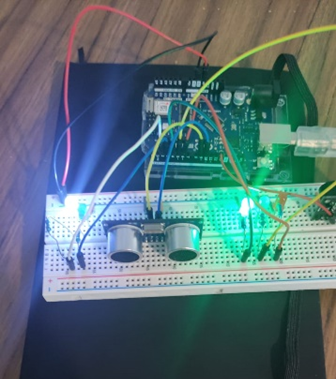
\includegraphics[scale=0.8]{img/eye1.png}}
\caption{Eye of Mordor}
\label{fig::eye1}
\end{figure}

To represent the animal we are using the card board also can be shown in the picture. As we can see in the Figure \ref{fig:eye23} (a) bellow, if we come near to the sensors it starts to read the cards(animals) presence and turn on the yellow LED and send the approximate distance to the hosting device, Figure \ref{fig:eye23}

\begin{figure}[!h]
\begin{subfigure}{.5\textwidth}
  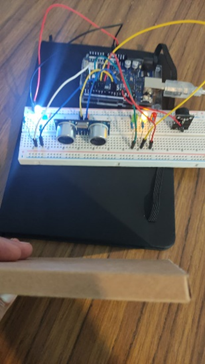
\includegraphics[width=.6\linewidth]{img/eye2.png}
  \caption{Reading Nearby animal}
  \label{fig:sub1}
\end{subfigure}%
\begin{subfigure}{.5\textwidth}
  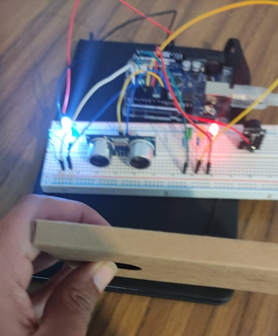
\includegraphics[width=.6\linewidth]{img/eye4.png}
  \caption{Reading Nearby animal}
  \label{fig:sub3}
\end{subfigure} \\ \\
\centering{
\begin{subfigure}{.5\textwidth}
  \centering{ 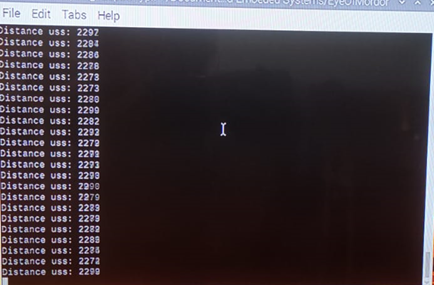
\includegraphics[width=.8\linewidth]{img/eye3.png}}
  \caption{User can check approximate distance}
  \label{fig:sub2}
\end{subfigure}
}
\caption{Eye of Mordor detection}
\label{fig:eye23}
\end{figure}

When it goes real close to the animal it turn on the red LED to notify user and send the distance info to the user so the user can know how close they are from the animal. This demonstration can be followed by the Figure \ref{fig:eye23}.

Once it gather the data it can forward it to its operator as shown in the Figure \ref{fig:eye23}. to ensure that there is an animal. Thus the operator can take necessary actions like whether to rescue, relocate or inform nearby farmer. The possibility is limitless.

Alternatively we can place A device like an “Alarm” or “Notification system on Smart phone” to alert the farmer that there is an animal so that he may take necessary precautions. To represent the scenario in our project, LED and Buzzers been used. Here in the presence of the Card (Animal) the buzzer makes noise and The LED Lights up to represent The Alarm and notification respectively. Once recognized the condition the user can turn off the buzzer and led by pressing the stop button on the smartphone app as shown in Figure \ref{fig:phone1}.

By realizing this system we believe, we will be able to save a lot of poor innocent souls from being a victim of Human advancement and interventions.




\begin{thebibliography}{9}
\bibitem{kanvanize}
Kanvanize. (n.d.). What Is Agile Project Management? A Comprehensive Guide. Kanban Software for Agile Project Management. https://kanbanize.com/agile/project-management

\bibitem{APM}
APM. (n.d.). Agile project management. What Is Agile Project Management? https://www.apm.org.uk/resources/find-a-resource/agile-project-management/

\bibitem{APM1}
APM. (n.d.-b). What is project management? https://www.apm.org.uk/resources/what-is-project-management/

\bibitem {github}
GitHub. (n.d.). About projects. About Projects. https://docs.github.com/en/issues/trying-out-the-new-projects-experience/about-projects

\bibitem {tech1}
DesPortes, K., Anupam, A., Pathak, N., and DiSalvo, B. (2016, June). BitBlox: a redesign of the breadboard. In Proceedings of The 15th International Conference on Interaction Design and Children (pp. 255-261). 

\bibitem{tech2}
Badamasi, Y. A. (2014, September). The working principle of an Arduino. In 2014 11th international conference on electronics, computer and computation (ICECCO) (pp. 1-4). IEEE

\bibitem{tech3}

Jolles, J. W. (2021). Broad‐scale applications of the Raspberry Pi: A review and guide for biologists. Methods in Ecology and Evolution, 12(9), 1562-1579.

\bibitem{tech4}

Mosquitto, E. (2018). Eclipse mosquitto. Eclipse Mosquitto. 


\end{thebibliography}

\end{document}